\documentclass[12pt, a4paper, hidelinks]{article}

\usepackage[icelandic]{babel}
\usepackage[T1]{fontenc}
\usepackage[utf8]{inputenc}


\usepackage{amsmath, amssymb, amsfonts}
\usepackage{mathtools}

\usepackage[outputdir=cache]{minted}
\usemintedstyle{default}
\renewcommand{\listingscaption}{Forrit}

\usepackage{url}
\usepackage{hyperref}
\usepackage[hang, flushmargin, bottom]{footmisc}

\usepackage[svgnames]{xcolor}
\usepackage{tabularx}
\usepackage{float}
\usepackage{graphicx}
\usepackage{booktabs}
\usepackage{enumerate}
\usepackage{multirow}
\usepackage{tikz}
\usetikzlibrary{arrows}
\usepackage{pifont}
\usepackage{multicol}
\usepackage{tcolorbox}
\usepackage{forest}

\usepackage{caption}
\usepackage{subcaption}

\newcommand{\cmark}{\color{Green}\ding{51}}
\newcommand{\xmark}{\color{Red}\ding{55}}

\usepackage{times, mathptmx}
\usepackage[scaled=0.85]{beramono}

\newenvironment{code}{\captionsetup{type=listing}}{}

\usepackage{fancyhdr}
\pagestyle{fancy}
\fancyhf{}
\fancyhead[L]{Kári Hlynsson}
\fancyhead[C]{TÖL203G Heimadæmi 11}
\fancyhead[R]{\today}
\fancyfoot[C]{\thepage}

\newcommand{\doctitle}{\uppercase{Heimadæmi 11}}
\newcommand{\coursename}{Tölvunarfræði 2}
\newcommand{\coursenum}{TÖL203G}

% ——— Mengjatákn
\newcommand{\N}{\mathbb{N}}
\newcommand{\Z}{\mathbb{Z}}
\newcommand{\Q}{\mathbb{Q}}
\newcommand{\R}{\mathbb{R}}
\newcommand{\C}{\mathbb{C}}

% ——— Vigrar
\renewcommand{\u}{\mathbf{u}}
\renewcommand{\v}{\mathbf{v}}
\renewcommand{\b}{\mathbf{b}}
\newcommand{\w}{\mathbf{w}}
\newcommand{\p}{\mathbf{p}}
\newcommand{\x}{\mathbf{x}}
\newcommand{\y}{\mathbf{y}}
\newcommand{\z}{\mathbf{z}}

% Define styles for nodes in the binary tree
\tikzset{
  binarytree/.style={
    draw,
    circle,
    thick,
    minimum size=0.75cm,
    inner sep=0pt,
    font=\sffamily\small
  },
  binaryedge/.style={
    draw,
    line width=1mm,
    red
  },
  binarytree empty/.style={
    draw=none,
    fill=none
  }
}

\graphicspath{{img}}

\begin{document}
\thispagestyle{plain}
\centerline{\bfseries\Large\doctitle}
\medskip
\centerline{\large\coursenum\ \coursename}
\bigskip

\centerline{\large Kári Hlynsson\footnote{Slóð á Github kóða: \url{https://github.com/lvthnn/TOL203G/tree/master/HD11}}}
\bigskip
\centerline{Háskóli Íslands}
\medskip
\centerline{\today}

\section*{Verkefni 1}
Í þessu dæmi gerum við ráð fyrir að Bellman-Ford reikniritið vinni með leggina í hækkandi röð eftir \emph{frá}-hnúti (þ.e. hnútinum $v$ í $v \to w$).
\begin{enumerate}[(a)]
    \item Hermið reiknirit Bellman-Ford á stefnunetinu hér fyrir neðan, með upphafshnútinn 3. Sýnið stöðuna á \texttt{distTo} eftir hverja umferð.

    \item Notið hugmyndina í (a)-lið til að útbúa stefnunet með $N$ hnútum þar sem reiknirit Bellman-Ford tekur $\Theta(N^2)$ tíma. Rökstyðjið keyrslutímann.
\end{enumerate}

\begin{figure}[H]
    \centering
    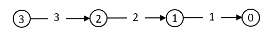
\includegraphics[width=0.75\textwidth]{HD11/pdf/img/V1.png}
    \label{fig:V1}
\end{figure}

\subsection*{Lausn}
\begin{enumerate}[(a)]
    \item Vegna þess að netið er keðja er enginn möguleiki á því að kall á \texttt{relax()} breyti gildi í \texttt{edgeTo} og \texttt{distTo} fyrir utan hina fyrstu umferð. Umferðirnar eru $|V| - 1 = 3$ talsins. Fylkið \texttt{distTo} er sett fram hér fyrir neðan eins og það leggur sig í lok hverrar umferðar.

    \begin{table}[H]
        \centering
        \caption{Staða \texttt{distTo} í upphafsstillingu}
        \begin{tabular}{lc}
            \toprule
            $v$ & \texttt{distTo[$v$]} \\
            \midrule
            3   & 0        \\
            2   & $\infty$ \\
            1   & $\infty$ \\
            0   & $\infty$ \\
            \bottomrule
        \end{tabular}
        \label{tab:my_label}
    \end{table}
    
    \begin{table}[H]
        \centering
        \caption{Staða \texttt{distTo} í umferð 1}
        \begin{tabular}{lc}
            \toprule
            $v$ & \texttt{distTo[$v$]} \\
            \midrule
            3   & 0        \\
            2   & 3         \\
            1   & 5 \\
            0   & 6 \\
            \bottomrule
        \end{tabular}
        \label{tab:my_label}
    \end{table}
    
    \begin{table}[H]
        \centering
        \caption{Staða \texttt{distTo} í umferð 2}
        \begin{tabular}{lc}
            \toprule
            $v$ & \texttt{distTo[$v$]} \\
            \midrule
            3   & 0        \\
            2   & 3         \\
            1   & 5 \\
            0   & 6 \\
            \bottomrule
        \end{tabular}
        \label{tab:my_label}
    \end{table}
    
    \begin{table}[H]
        \centering
        \caption{Staða \texttt{distTo} í umferð 3}
        \begin{tabular}{lc}
            \toprule
            $v$ & \texttt{distTo[$v$]} \\
            \midrule
            3   & 0        \\
            2   & 3         \\
            1   & 5 \\
            0   & 6 \\
            \bottomrule
        \end{tabular}
        \label{tab:my_label}
    \end{table}
    
    \item Rifjum upp að tímaflækja Bellman-Ford reikniritsins er $\Theta(|E||V|)$. Sé stefnunetið ámóta keðju eins og í (a)-lið er fjöldi leggja $|V| - 1$. Sé $|V| = N$, þá fæst $|E| = N - 1$ og því er tímaflækjan
    $\Theta\big(N(N - 1)\big)$ það er að segja $\Theta(N^2)$. Þannig er stefnunet sem uppfyllir þetta skilyrði útbúið með því að tengja hnútana í línulegri röð, eins og í dæmi (a).
\end{enumerate}

\newpage

\section*{Verkefni 2}
Segjum að við höfum stefnunet $G$ með þyngdum á leggjum. Stystu vegir hafa verið fundnir fyrir $G$ frá upphafshnúti $s$. Ef við bætum við fasta $K$ við þyngdir allra leggja $G$ þá er ekki víst að stystu vegirnir séu þeir sömu og áður. Sýnið dæmi um net þar sem þetta gildir og rökstyðjið það. Þið megið ráða þyngdum einstakra leggja og gildinu á $K$.

\subsection*{Lausn}
Ímyndum okkur að mengi leggja sé á forminu þrennda $(v, w, \omega)$ þar sem $\omega$ er þyngd leggjarins en fyrri tvö stökin frá- og eftir-hnútarnir. Við viljum smíða net sem hefur neikvæða þyngd $w_i$ þannig að hliðrun þyngdanna um $K$ þ.e. aðgerðin $E \oplus (0, 0, K)$ hafi í för með sér að stysti vegur breytist. Mynd fyrir neðan sýnir dæmi um slíkt net.

\begin{figure}[H]
    \centering
    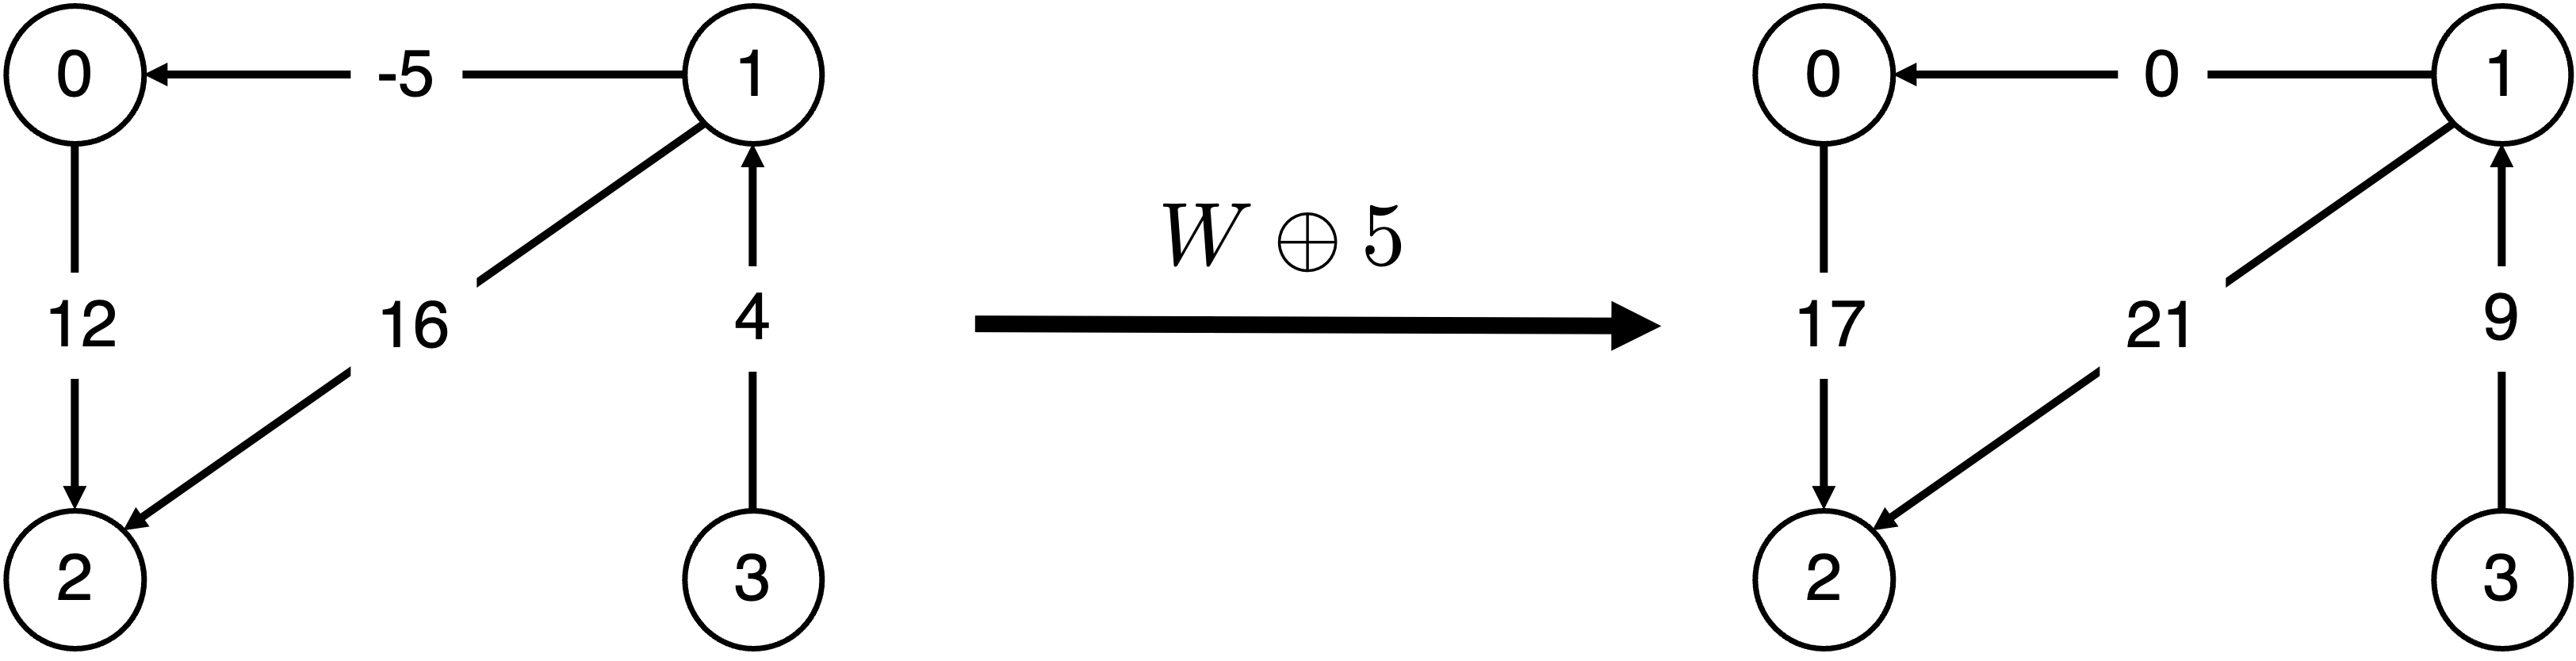
\includegraphics[width=\textwidth]{HD11/pdf/img/V2-soln.png}
    \caption{Umbeðið stefnunet.}
    \label{fig:V2-soln}
\end{figure}
\noindent
Við sjáum að á vinstri hliðinni samanstendur stysti vegurinn frá $0$ til $2$ af $0 \to 1$ og
$1 \to 2$ með þyngdina $-0.5 + 1.6 = 1.1$, en eftir hliðrun er stysti vegurinn einfaldlega $0 \to 2$ með þyngd $1.7$.

Ef $K$ er valið þannig að það núlli neikvæðu þyngdina út hættir hún að hafa áhrif á lengd vegarins og þá er ''ávinningurinn'' af þeirri aðgerð enginn. Hins vegar þyngist leggurinn sem neikvæða þyngdin núllaði út og það kann að leiða til þess að annar styttri vegur tekur forystu.

\newpage

\section*{Verkefni 3}
Gefið er stefnunetið fyrir neðan. Rekjið ykkur í gegnum reiknirit Dijkstra með upphafshnút 0. Sýnið í hvaða röð hnútarnir eru settir í stysta-vegar tréð og fyrir hvern hnút rökstyðjið í nokkrum orðum hvers vegna hnúturinn kemur inn í tréð á þessum tíma.

\begin{figure}[H]
    \centering
    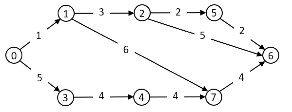
\includegraphics{HD11/pdf/img/V3.png}
    \label{fig:V3}
\end{figure}

\subsection*{Lausn}
Myndirnar hér fyrir neðan sýna hvernig reikniritið bætir við í tréð, ásamt ástandi \texttt{distTo} fylkisins og biðraðarinnar \texttt{pq}.

\begin{figure}[H]
    \centering
    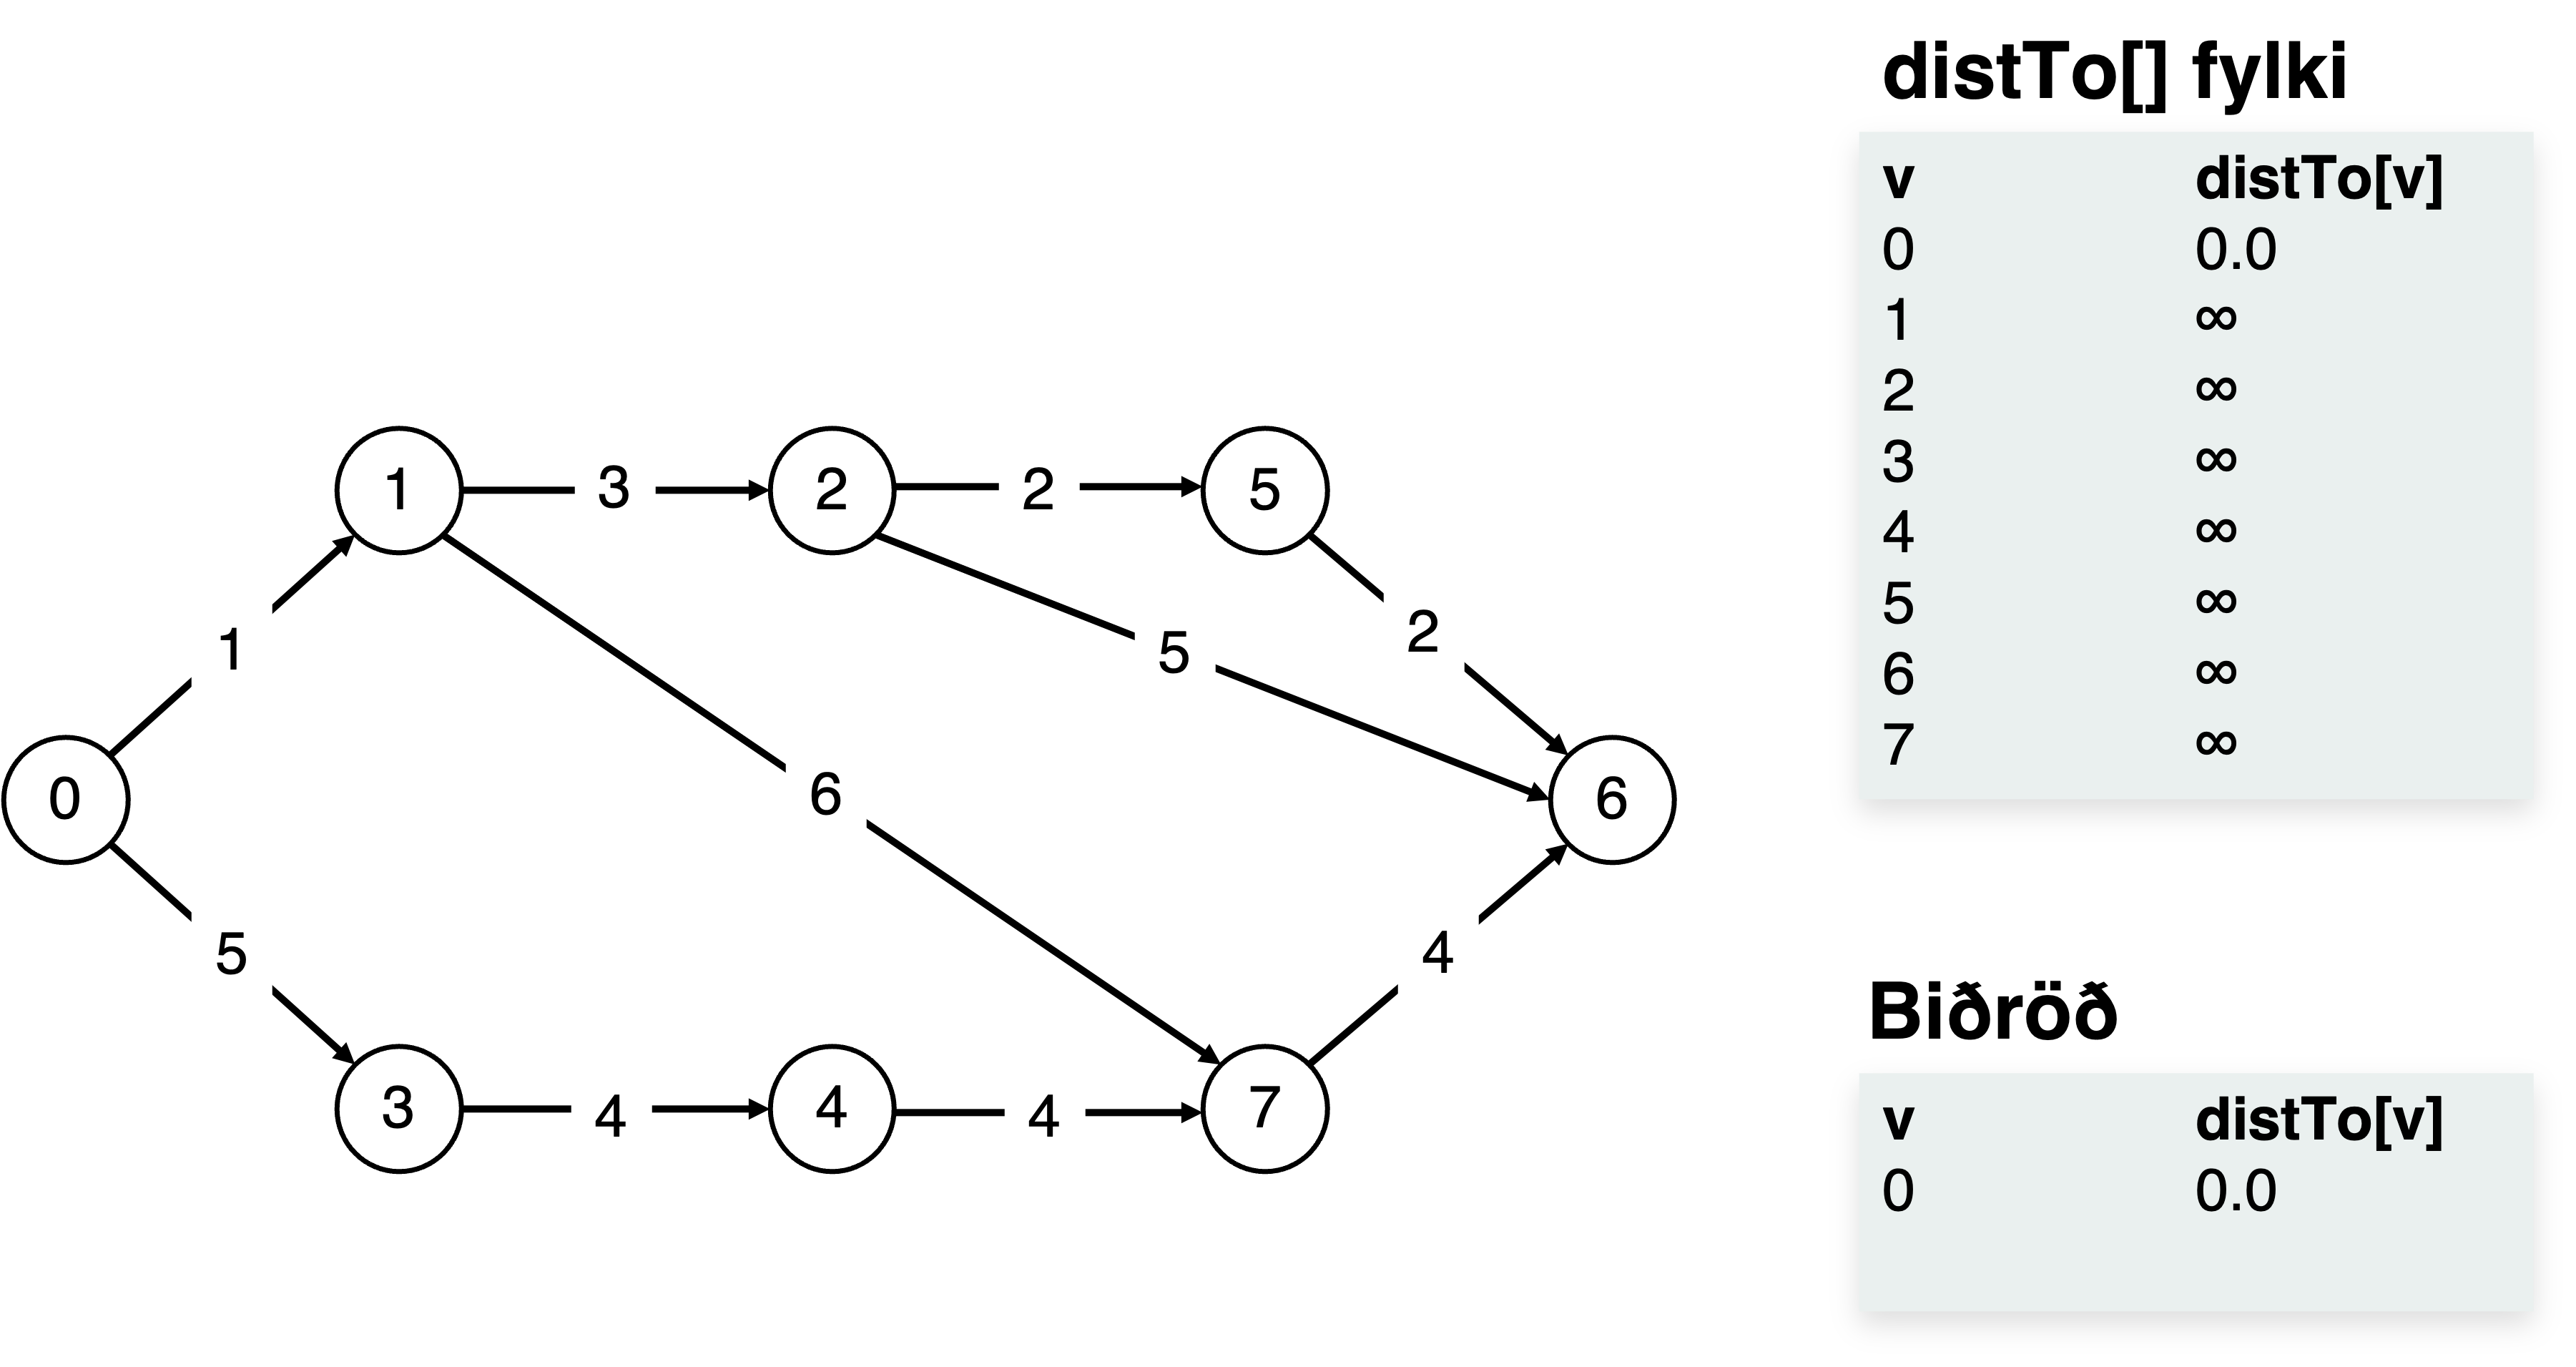
\includegraphics[width=\textwidth]{HD11/pdf/img/dijkstra/im1.png}
    \label{fig:dijkstra1}
\end{figure}

\begin{figure}[H]
    \centering
    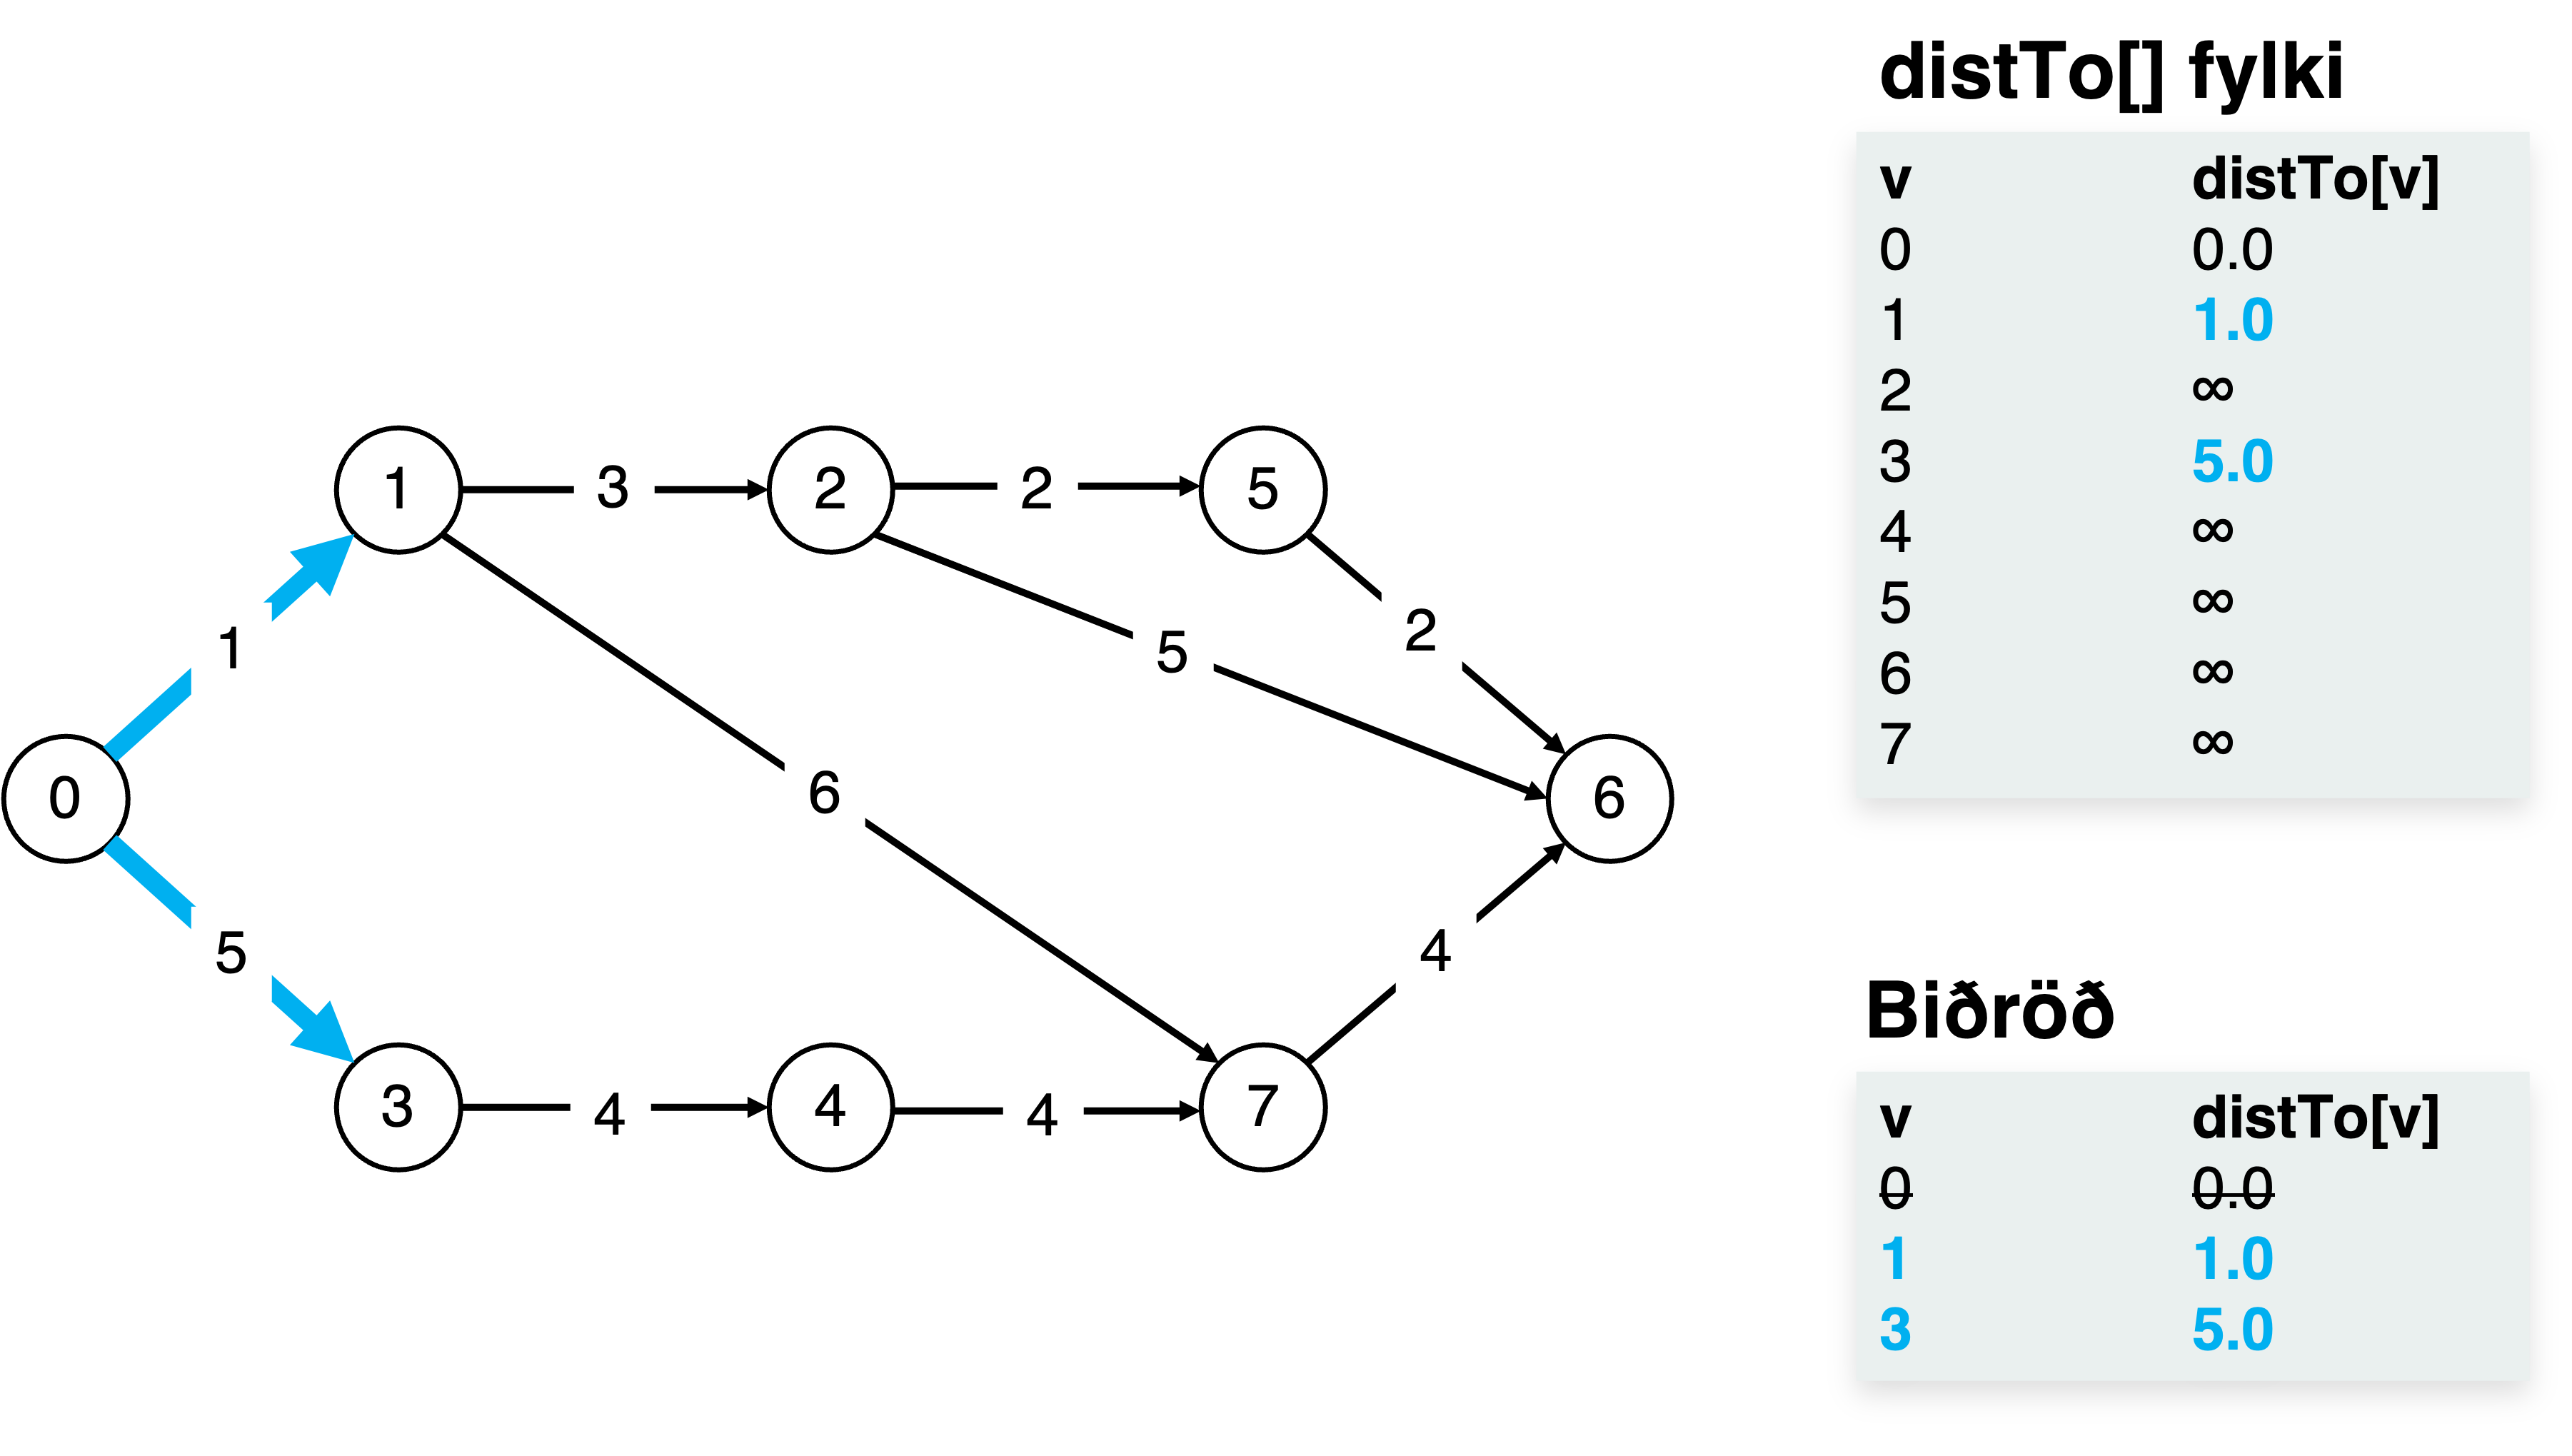
\includegraphics[width=\textwidth]{HD11/pdf/img/dijkstra/im2.png}
    \label{fig:dijkstra2}
\end{figure}

\begin{figure}[H]
    \centering
    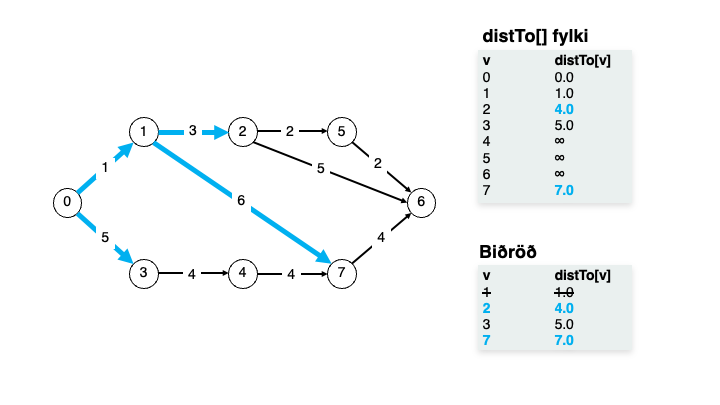
\includegraphics[width=\textwidth]{HD11/pdf/img/dijkstra/im3.png}
    \label{fig:dijkstra3}
\end{figure}

\begin{figure}[H]
    \centering
    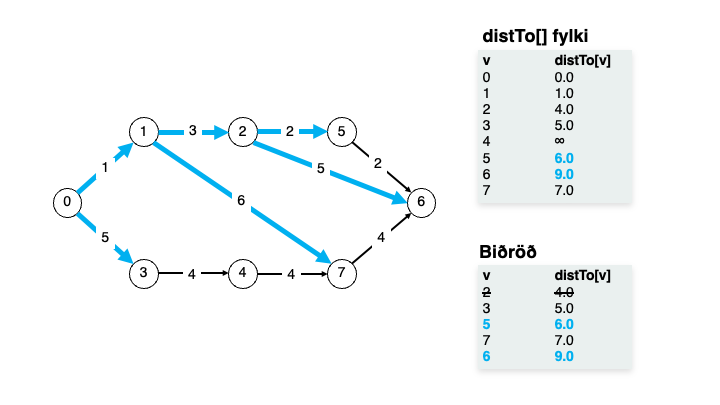
\includegraphics[width=\textwidth]{HD11/pdf/img/dijkstra/im4.png}
    \label{fig:dijkstra4}
\end{figure}

\begin{figure}[H]
    \centering
    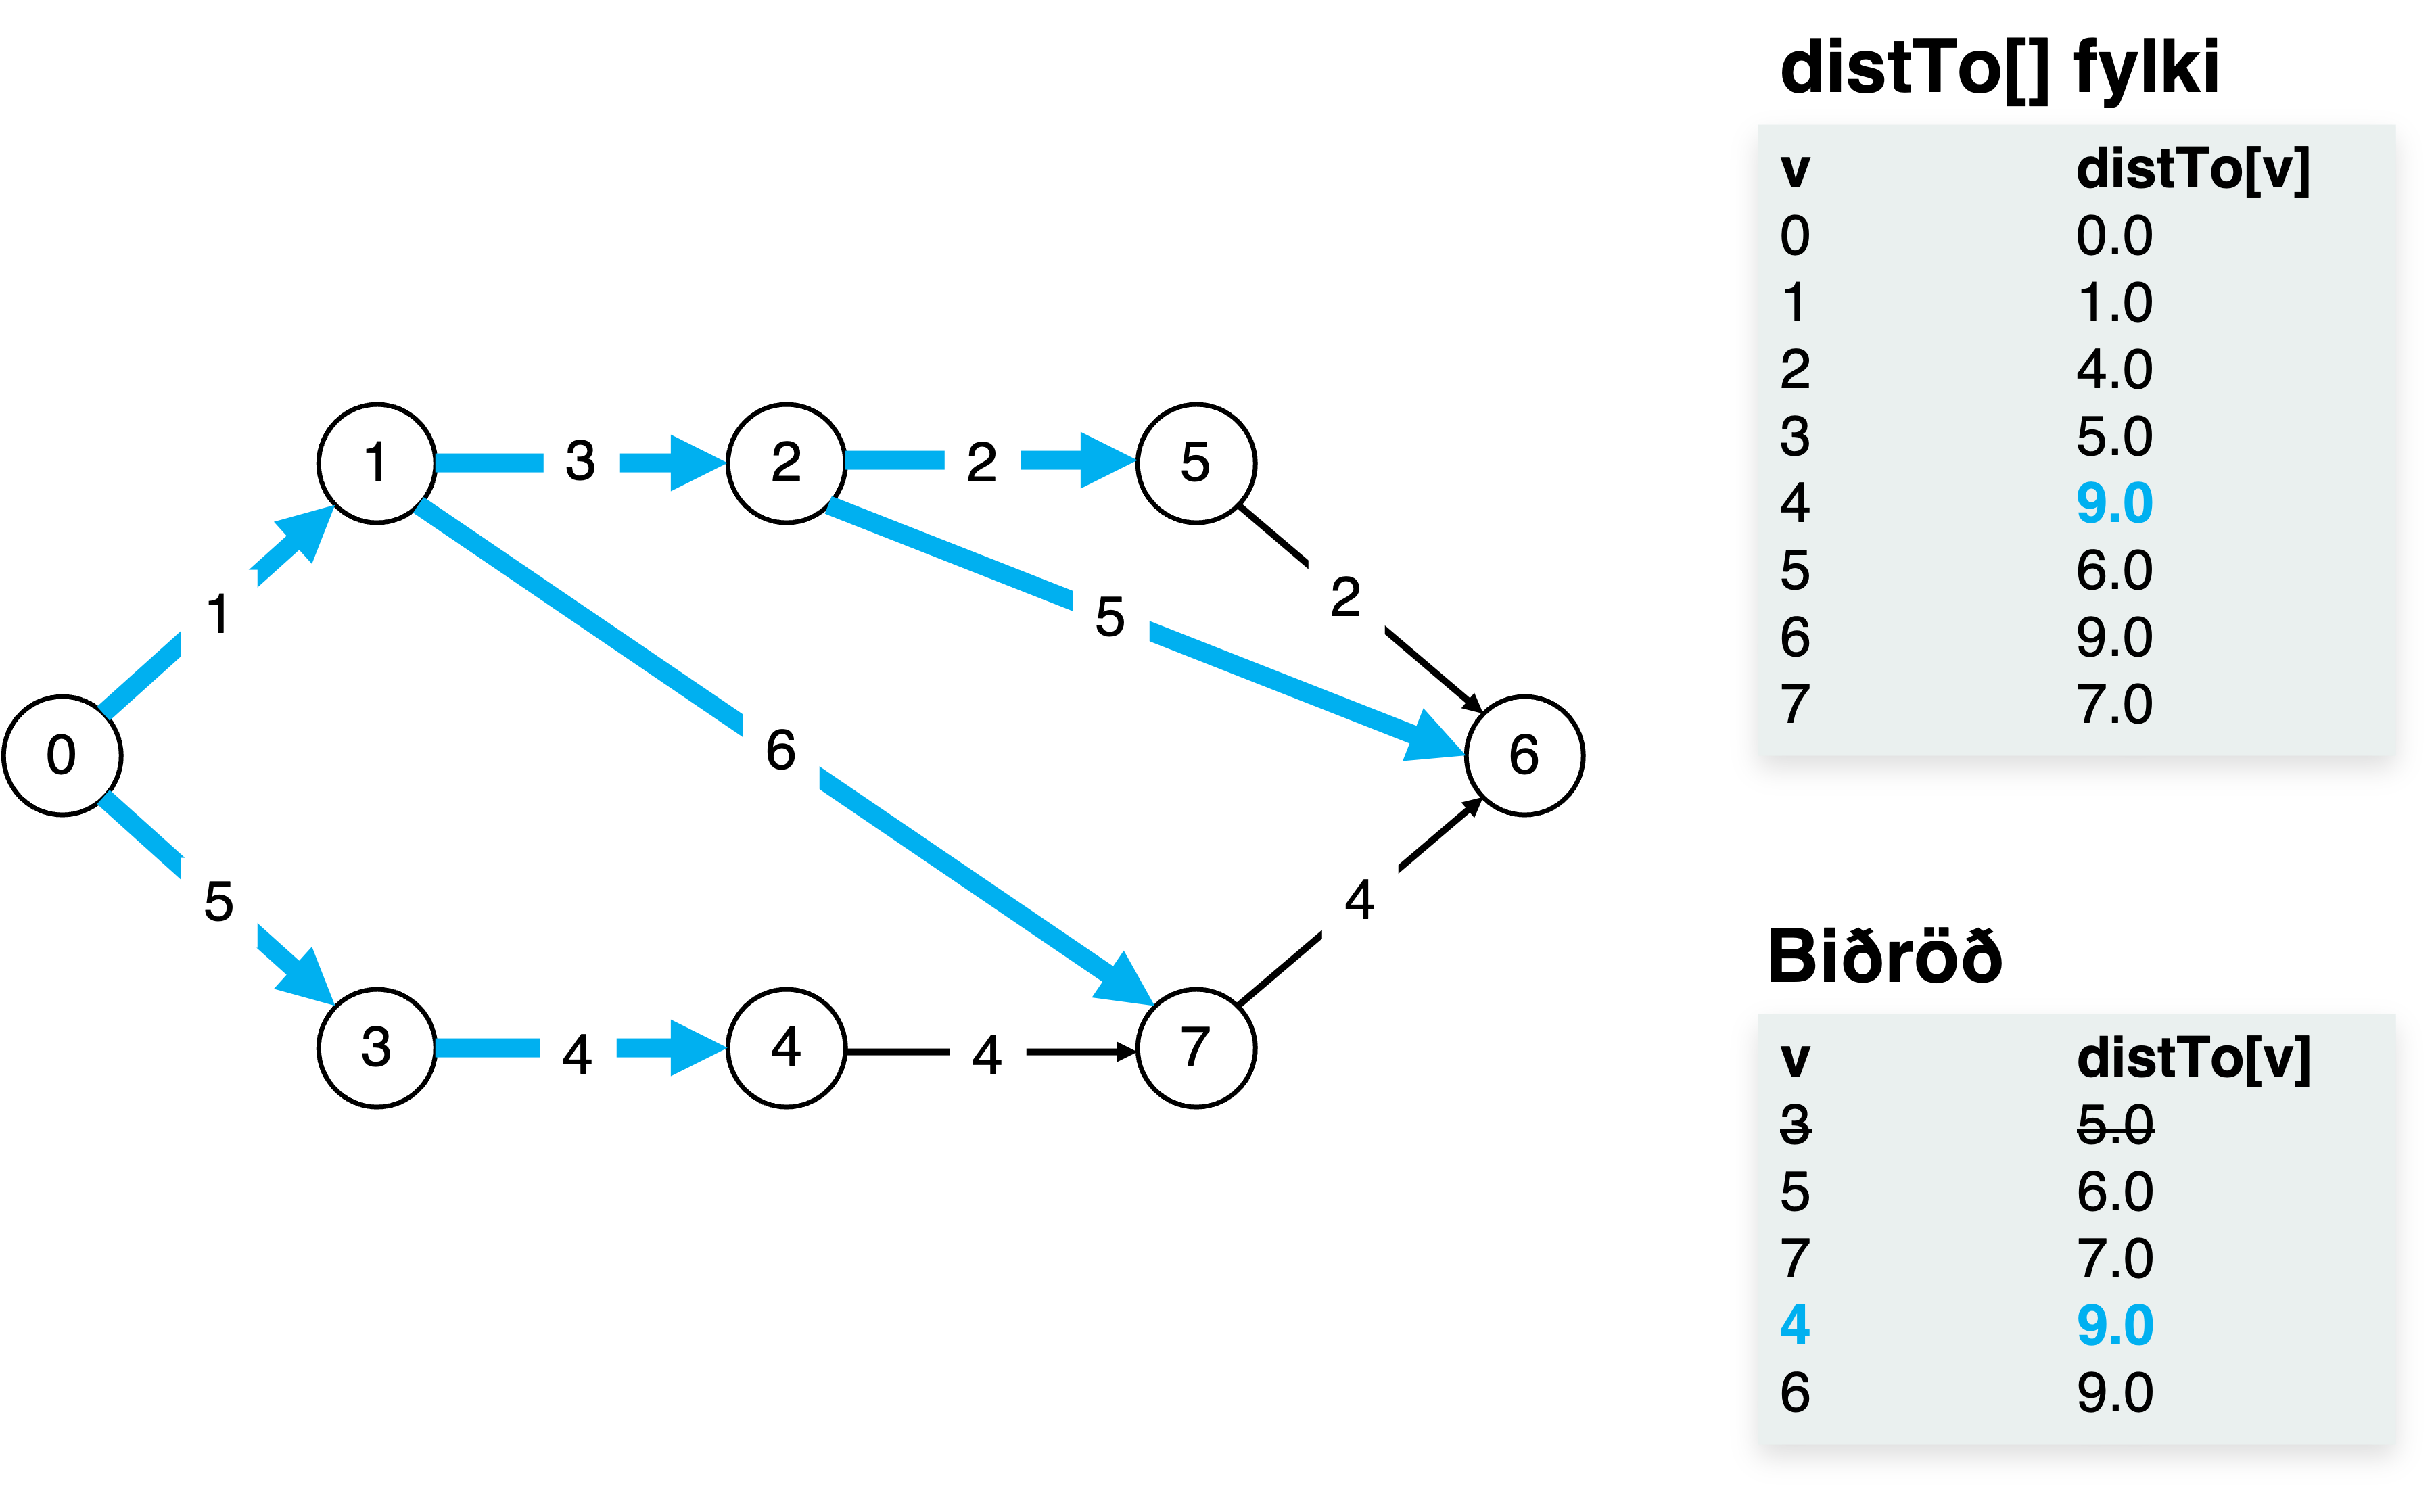
\includegraphics[width=\textwidth]{HD11/pdf/img/dijkstra/im5.png}
    \label{fig:dijkstra5}
\end{figure}

\begin{figure}[H]
    \centering
    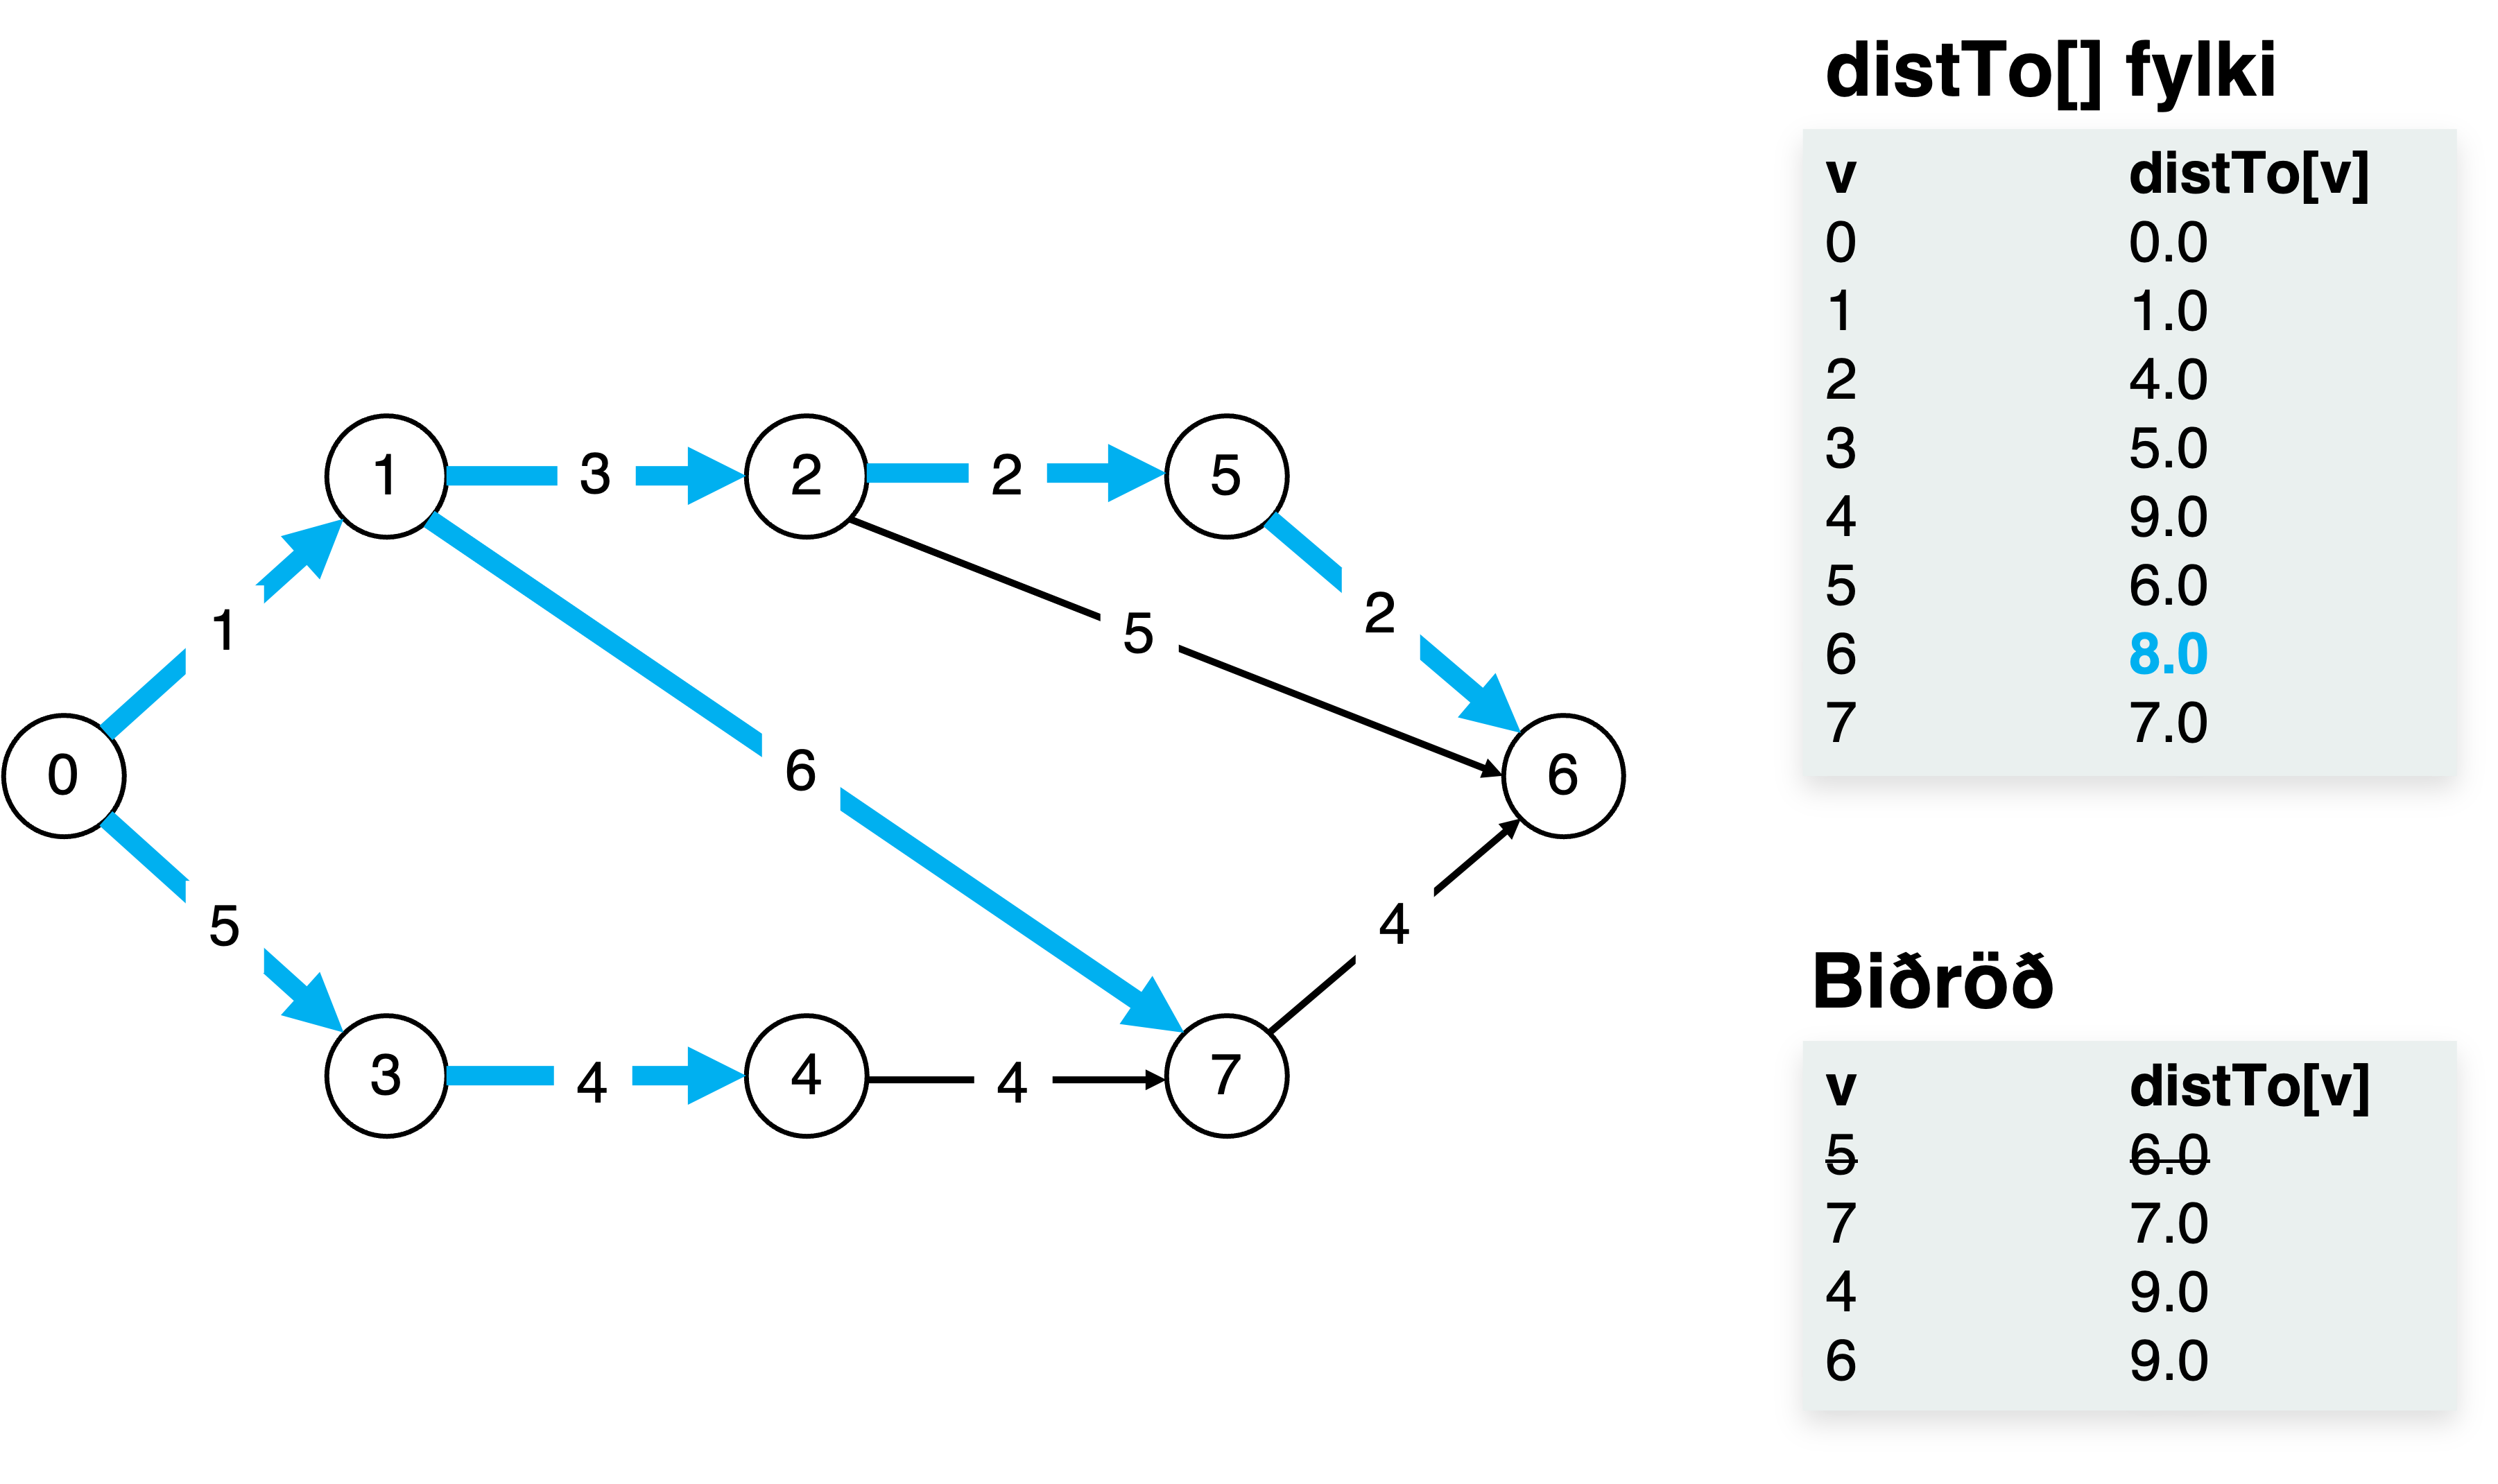
\includegraphics[width=\textwidth]{HD11/pdf/img/dijkstra/im6.png}
    \label{fig:dijkstra6}
\end{figure}

\begin{figure}[H]
    \centering
    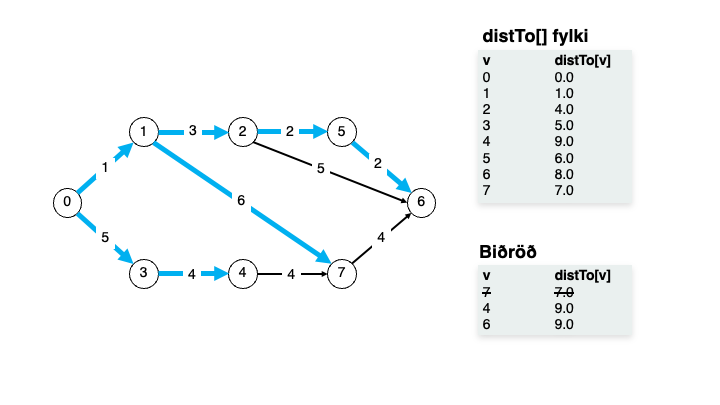
\includegraphics[width=\textwidth]{HD11/pdf/img/dijkstra/im7.png}
    \label{fig:dijkstra7}
\end{figure}


\begin{figure}[H]
    \centering
    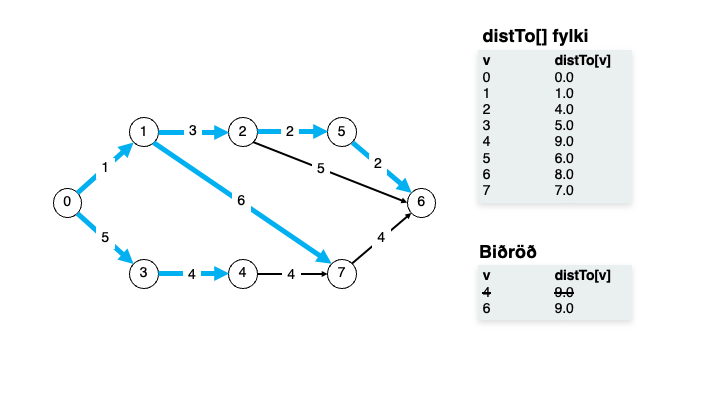
\includegraphics[width=\textwidth]{HD11/pdf/img/dijkstra/im8.png}
    \label{fig:dijkstra8}
\end{figure}

\begin{figure}[H]
    \centering
    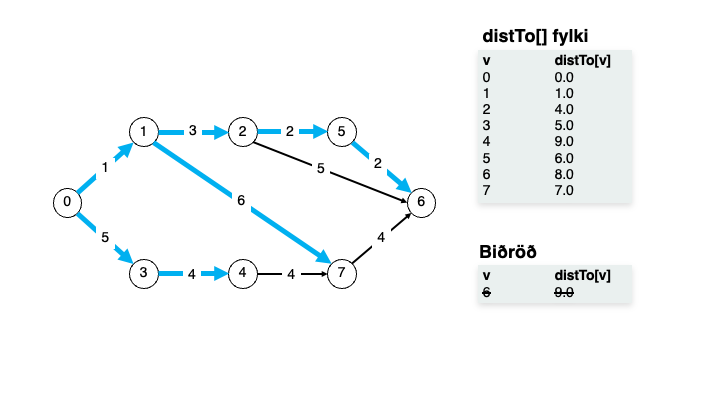
\includegraphics[width=\textwidth]{HD11/pdf/img/dijkstra/im9.png}
    \label{fig:dijkstra9}
\end{figure}

\begin{figure}[H]
    \centering
    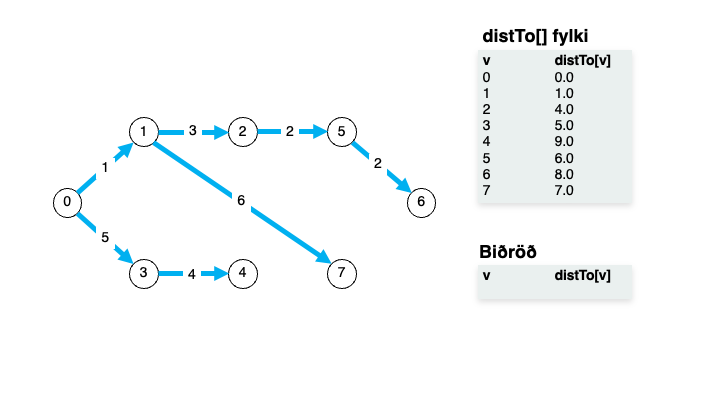
\includegraphics[width=\textwidth]{HD11/pdf/img/dijkstra/im10.png}
    \label{fig:dijkstra10}
\end{figure}

\noindent
Á seinni myndinni á bls. 6 verður slökun þ.a. \texttt{distTo[6]} minnkar.

\newpage

\section*{Verkefni 4}
Sýnið stefnunet með þyngdir á leggjum, þar sem ein þyngdin er neikvæð, en
reiknirit Dijkstra gefur samt rétta útkomu. Netið þarf að hafa a.m.k. 4 hnúta.
Rökstyðjið það að reikniritið gefi rétta útkomu.

\subsection*{Lausn}
Umbeðið stefnunet er sýnt fyrir neðan á mynd. Hér gerum við ráð fyrir að $2$ sé upphafshnúturinn þegar reikniritið er keyrt.

\begin{figure}[H]
    \centering
    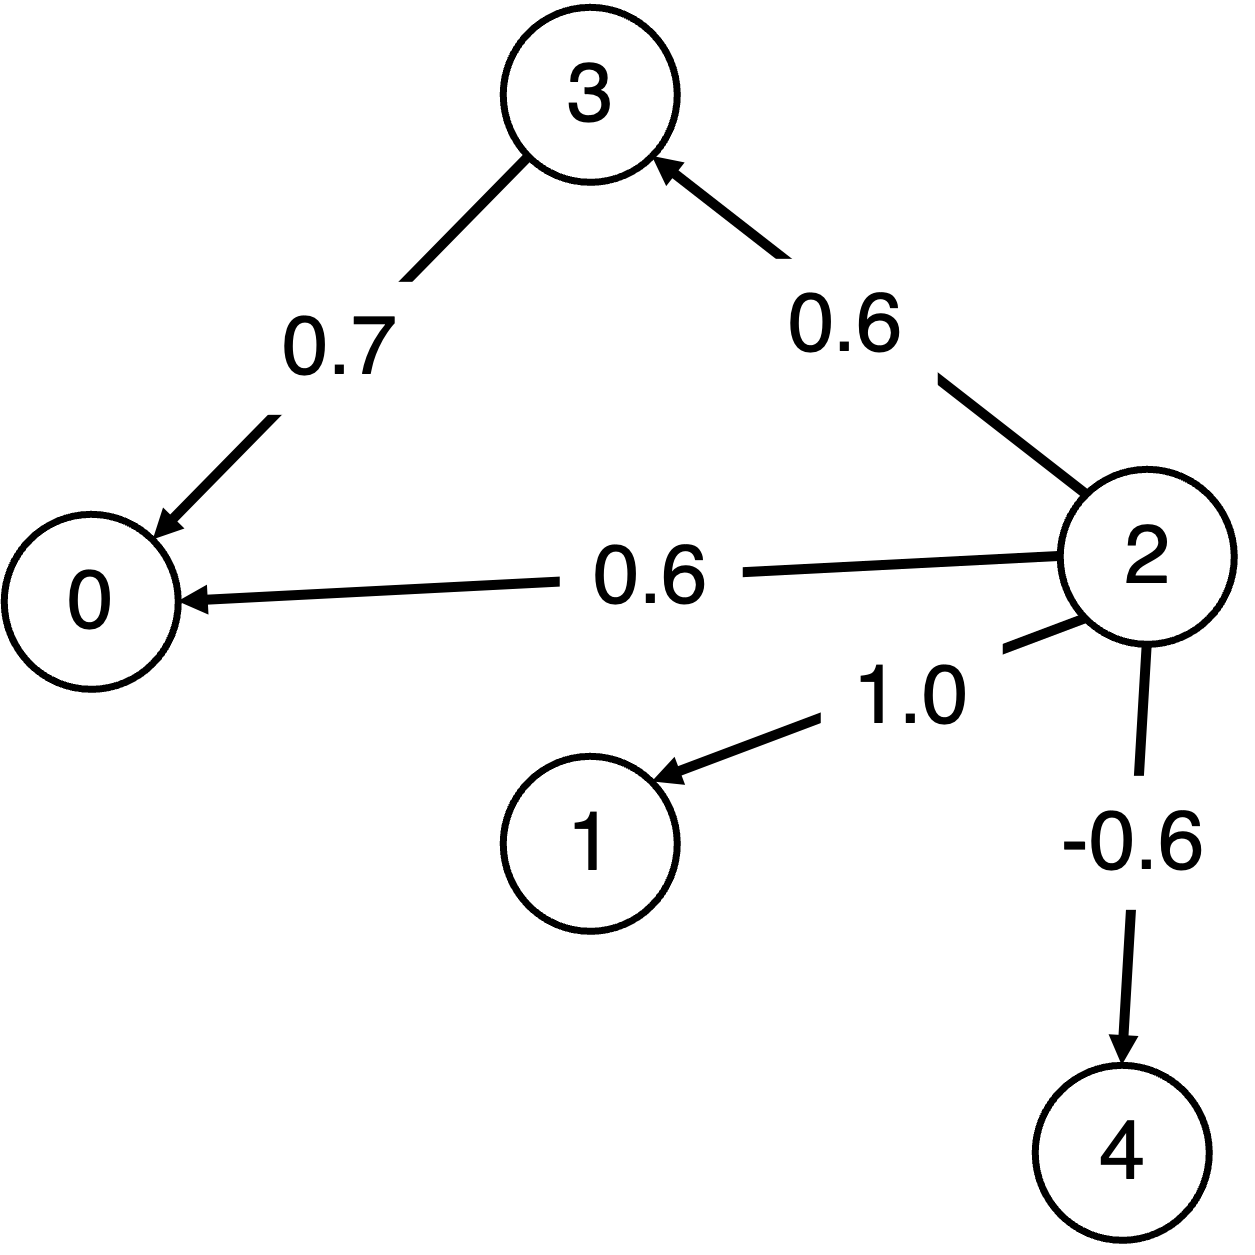
\includegraphics[width=0.65\textwidth]{HD11/pdf/img/dijkstra/dijkstra-negative-correct.png}
    \caption{Stefnunet með neikvæðum legg þar sem Dijkstra skilar réttri niðurstöðu}
    \label{fig:dijkstra-negative}
\end{figure}

\noindent
Þyngd leggjarins $2 \to 4$ er neikvæð en reikniritið skilar samt réttri niðurstöðu því stysti vegur frá $2$ til $4$ getur bara verið neikvæði leggurinn. Hann hefur jafnframt engin áhrif á hina vegina og því kemst reikniritið að réttri niðurstöðu.
\end{document}
